\chapter{TRAX Fault Model}
\label{chap:trax}

In the context of digital circuit testing, a fault model is an abstraction of a class of defects, created to simplify their characteristics in order to make analysis more tractable.
%
Fault models are particularly useful for understanding the high-level impact of a defect on circuit behavior.
%
The simplest fault model, the single stuck-line (SSL) model~\cite{abramovici90}, assumes each individual signal line is susceptible to becoming permanently stuck at either logic-low or logic-high.
%
Another fault model, the bridge fault model~\cite{abramovici90}, hypothesizes that two signals are errantly connected.
%
Depending on the relative drive strengths of the two bridged signals the stronger may override the weaker, or the two signals may form a wired-AND or wired-OR logic function.

The choice of fault model is largely a tradeoff between how closely a fault model matches the targeted defects and the size of the fault universe.
%
Simpler fault models such as the SSL have a relatively small fault universe ($2 n$, where $n$ is the number of circuit signal lines), while more complex fault models like the bridge model have a larger fault universe (for $m$-line bridges, on the order of $m^n$i, in theory).
%
In general, the preferred fault model for any particular situation is the fault model that best captures the expected effects of the targeted defects while still having a sufficiently small fault universe.

In this thesis, the targeted defects are early-life and wear-out failures.
%
Early-Life Failures (ELF) are caused by latent manufacturing defects not detected by factory tests, such as gate-oxide defects~\cite{chen08}.
%
Chips affected by ELF can fail early in their lifetime, often much sooner than the specified product lifetime.
%
ELF-affected transistors will experience gradual delay increases over time before functional failures occur.
%
Wear-out failures include mechanisms like Negative Bias Temperature Instability (NBTI), which changes the threshold voltage of a PMOS transistor, resulting in decreased transistor drive current, ultimately leading to circuit-speed degredation~\cite{borkar06,schroder03}.
%
NBTI first became a significant issue at the 90nm technology node~\cite{agarwal07} but worsens as technology continues to scale~\cite{reddy02}.
%
Various experiments involving actual test chips~\cite{agarwal07,chen09} demonstrate that both early-life and wear-out failures manifest as delay increases in standard cells.

\section{Existing Fault Models}
\label{sec:trax_existing_fault_models}

There are a variety of fault models targeting changes in circuit delays, such as those caused by early-life and wear-out failures.
%
For example, the path delay fault model~\cite{smith85,lin87} characterizes a delay-causing defect as an accumulation of additional path delay through the circuit from a primary input to a primary output.
%
This model, however, suffers from the fact that the number of path-delay faults can be exponential in the number of circuit lines~\cite{heragu96}, leading to a large fault universe.
%
The segment delay fault model~\cite{heragu96}, on the other hand, is a parameterized fault model that models delay as distributed along a short segment (of length $L$) of a path, where the parameter $L$ is chosen based on defect statistics.
%
The size of the fault universe can be controlled by the choice of $L$.
%
Other delay fault modules include the Transition Path Delay Fault model~\cite{pomeranz08tpdf}, the Propagation Delay Fault model~\cite{lin05}, and the Inline Resistance Delay Fault model~\cite{benware04}.
%
An ideal fault model to represent the slowdown caused by early-life and wear-out failures is the gate delay fault (GDF) model~\cite{jha03}.
%
Detection of a GDF requires producing a transition at the affected gate output and sensitizing a circuit path from the gate to one or more primary outputs.
%
A GDF will only be detected if the additional delay due to the fault is larger than the slack of a path appropriately sensitized.
%
Identifying a test to detect a GDF is thus an optimization problem that involves searching for a sensitizable path through the gate that exhibits the minimal slack.
%
Optimization adds undesired complexity to the already intractable test generation process, making deployment of the GDF model for use in a dictionary much more challenging.

The most commonly-deployed delay fault model is the transition fault (TF) model~\cite{jha03}.
%
It is widely used because it is a delay fault model with a limited fault universe and very related to the ubiquitous SSL fault model~\cite{wang14}.
%
Whereas the GDF model makes no assumption about the increase in delay, the TF model, on the other hand, assumes the delay to be larger than the slack of any sensitized path through the fault site.
%
This assumption significantly reduces complexity because any test that sensitizes a path from the fault site to an observable point will detect a TF fault.
%
That is, test generation remains a satisfiability problem as opposed to an optimization problem.
%
The TF model is more tractable but is very pessimistic since it implicitly assumes that every fault will produce errors at the output of each sensitized path.%todo add wang14 to intro trax section

The unspecified-transition fault (UTF) model~\cite{pomeranz08} is a compromise between the gate delay fault model and the transition fault model.
%
The UTF model makes no assumptions about the length of the delay and represents the uncertainty in fault delay through the use of the unknown value \textit{X}, produced when a UTF is activated.
%
While the GDF model makes no assumptions about delay size, and the TF model assumes a worst-case gross delay, the UTF exists as a compromise, using the \textit{X} value to represent the uncertainty of the modeled delay.
%
This chapter of the dissertation details an enhancement of the UTF model that includes activation and propagation due to glitches resulting from hazards, noise\footnote{Due to limitations in the gate-level Verilog simulations used to generate circuit responses from injected delays, we do not consider noise-based activation.}, etc.
%
We refer to this new fault model as the Transition-X (TRAX) fault model.

\section{TRAX Fault Model}
\label{sec:trax_trax}

Similar to a transition fault, a TRAX fault is either a slow-to-fall (STF) or slow-to-rise (STR) fault, and is activated by either a transition of the correct polarity (1-to-0 or 0-to-1, respectively) or due to a glitch.
%
Activation-by-glitch is the prime difference between the TRAX and the unspecified-transition fault models.
%
Simulation experiments (designed to mimic slow-downs due to aging) revealed that some failing responses could not be explained by any UTF.
%
Further investigation revealed the source of this discrepancy, namely that signal glitches activated the injected rising or falling delays.
%
This situation is not covered by the conventional transition-based fault activation used by TF and UTF, and the TRAX fault model is developed to also include glitch-based fault activation.
%
This enhancement ensures that TRAX fault effects subsume the effects of a co-located delay defect.

A glitch is an undesired and transient pulse in a signal, typically generated at the output of a gate driven by two successive sets of inputs that do not provide a constant controlling input\footnote{A glitch can also be created by excessive noise in cross-coupled on-chip interconnects~\cite{cuviello99}, but noise is not considered in this work due to limitations of the gate-level Verilog simulation employed.}.
%
To explain this concept further, we first need some background:

\begin{itemize}
\item In the two-vector test scheme employed in this work, each test consists of two test vectors, referred to as $V_1$ and $V_2$.
\item Many gate types have a ``controlling input'' that forces the gate output to a certain value regardless of the other gate inputs.
%
For example, the controlling input value for a NAND gate is logic-low; any low input will force the gate output high.
%
XOR and XNOR gates do not have a controlling input value.
\item A controlling input is ``constant'' if at least one of the gate inputs is driven with a constant controlling value in both $V_1$ and $V_2$.
\end{itemize}

For a two-input NAND gate $Y = \overline{(A \land B)}$, the inputs ($A = 0 \rightarrow 0$, $B = 1 \rightarrow 0$) provide a constant controlling value (logic-low) to input $A$, leading to a constant gate output of ($Y = 0 \rightarrow 0$).
%
In contrast, for the inputs ($A = 0 \rightarrow 1$, $B = 1 \rightarrow 0$), even though the expected output is also ($Y = 0 \rightarrow 0$), there exists the potential of a gate output glitch ($Y = 0 \rightarrow 1 \rightarrow 0$) due to the lack of a constant controlling input.
%
Such a test pair, with no constant controlling input, is referred to as a \textit{hazardous} test pair, given the potential for a glitch on the gate output.
%
In the TRAX fault model, where all faults are placed at gate outputs, a fault can be activated by a glitch due to a coincident hazard.
%
The hazard condition is added as a fourth logic value for TRAX fault simulation, resulting in a four-valued algebra of \verb+{0, 1, X, H}+.
%
The extended truth tables for the eight primitive gates are shown in Figure~\ref{fig:trax_gate_evaluation}.

%\vskip 0.5em%
\begin{figure}[htbp]
\centering
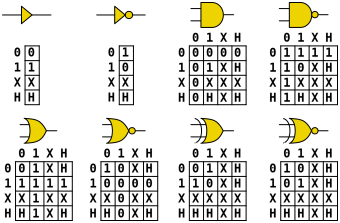
\includegraphics[width=0.8\columnwidth]{fig_gate_evaluation}
\caption{Truth tables for the eight primitive gate types are extended to support the four-value logic of the TRAX fault model.}
\label{fig:trax_gate_evaluation}
\end{figure}
%\vskip 0.5em%

An advantage of the TRAX fault model is that the \textit{X} value captures all the possible transport-delay changes that can be exhibited by a gate affected by NBTI or ELF since the propagation of the \textit{X} value is conservative.
%
Whereas the errors from a conventional transition fault could interact to either increase or reduce the number of fault-effect observations (i.e., failing outputs), the use of the \textit{X} value can only increase the number of failing outputs.
%
In other words, the set of sensitized paths with \textit{X} values will subsume the sensitized paths associated with any GDF of any delay.
%
In addition, any error cancelling due to fault masking that may occur due to the TF fault model is not possible in the TRAX fault model.

The ISCAS85 benchmark circuit c17 \cite{brglez85} shown in Figure~\ref{fig:trax_c17_tf_trax} is used to contrast the TF and TRAX models.
%
TF and TRAX faults are simulated at both sites $F_1$ and $F_2$, using two test-vector tests.
%
Table~\ref{table:trax_tf_trax_comparison} shows how fault effects propagate from each fault site to the circuit outputs.
%
The first pair of vectors activates a slow-to-fall fault at $F_1$; both the TF and TRAX produce a faulty value on the lower output $g$.
%
For this case, both faults are detected and produce the same response.
%
The second pair of vectors activates a slow-to-rise fault at $F_2$.
%
Here, more complex behavior arises, demonstrating the difference between TF and TRAX.
%
For TF, the reconvergent fanout logically masks the slowed transitions reaching the upper output $f$.
%
Masking is not possible for TRAX, resulting in both outputs having \textit{X} values, which subsumes the response of the TF.
%
The \textit{X} values at the two outputs mean it is possible that the actual response of a slowdown could subsume, match, or mismatch the TF response.

%\vskip 0.2em%
\begin{figure}[hbtp]
\centering
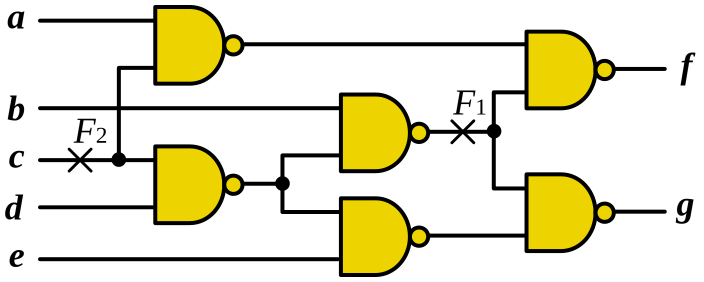
\includegraphics[width=0.8\columnwidth]{fig_c17_tf_trax}
\caption{Contrasting fault-effect propagation for the TF and TRAX models.}
\label{fig:trax_c17_tf_trax}
\end{figure}
\begin{table}[htbp]
\renewcommand{\arraystretch}{1.3}% increase table row spacing, adjust to taste
\centering
\begin{tabular*}{0.9\columnwidth}{@{\extracolsep{\fill}}r|r|r|c|c|c}
Fault&Fault&Two-vector test&\multicolumn{3}{c}{Output: $f g$}\\
site&type&($v_1$, $v_2$): $a b c d e$&FF&TF&TRAX\\
\hline
\multirow{2}{*}{$F_1$}&\multirow{2}{*}{STF} &$v_1: 10100$&10&10&10\\
                      &                     &$v_2: 11100$&11&10&1X\\
\hline
\multirow{2}{*}{$F_2$}&\multirow{2}{*}{STR} &$v_1: 11010$&11&11&11\\
                      &                     &$v_2: 11110$&10&11&XX\\
\end{tabular*}
\caption{Fault-free (FF) behavior of benchmark circuit c17 \cite{brglez85} (Figure~\ref{fig:trax_c17_tf_trax}) compared to TF and TRAX faults located at sites $F_1$ and $F_2$.}
\label{table:trax_tf_trax_comparison}
\end{table}
%\vskip 0.2em%

Fault simulation of TRAX faults is very similar to the TF model.
%
Instead of assuming a grossly-slowed transition, an \textit{X} value is injected when a TRAX fault is activated, either by a conventional transition or by a hazard value.
%
These injected \textit{X} values are propagated through the simulated circuit, producing the fault-free values of 0, 1, or the potentially faulty value \textit{X} at the observation points.
%
Additionally, a TRAX-without-hazards fault model variant (which is equivalent to the UTF model), where a fault can only be activated by a conventional transition, is also used in later sections to evaluate fault dictionary size (Section~\ref{sec:dict_exp_size_res}) and on-chip diagnosis effectiveness (Section~\ref{sec:diag_exp_traxnh}).

Interpretation of observed \textit{X} values at the outputs of the circuit under test requires further discussion.
%
Observed \textit{X} values resulting from TRAX fault simulation identify outputs that could, but not necessarily, be affected by a slowdown at the fault site.
%
In other words, outputs that have \textit{X} values may or may not exhibit an error, depending on the level of slowdown.
%
It is assumed for every test that detects a given TRAX fault that at least one observed \textit{X} value will actually be erroneous, guaranteeing detection.
%
Since no knowledge about the timing is assumed, it cannot be known a priori however which output will take on an incorrect value when a TRAX fault is detected.
%
Due to this uncertainty, the set of potentially-faulty outputs for a particular fault-test pair tells a different tale than the fault simulation responses of a conventional fault model.
%
For example, the fault simulation output for a particular transition fault describes how the circuit would behave if it were affected by a gross-delay defect located at the same point in the circuit as the modeled fault.
%
In contrast, the uncertainty as to which TRAX potentially-faulty outputs actually produce a faulty output means that it does not describe the expected response of a co-located defect.
%
Instead, the set of potentially-faulty outputs for a TRAX fault-test pair describes which circuit outputs \textit{could} be affected by a co-located defect.
%
This is a subtle point that supports the general-purpose nature of the TRAX fault model.
%
Effectively, TRAX fault simulation captures the relationship between incorrect circuit outputs and the set of modeled TRAX faults that could have caused that faulty behavior.
%
This enables TRAX to handle not just defects that increase delay, but also defects that decrease delay.


\section{GPU-Accelerated TRAX Fault Simulation}
\label{sec:trax_gpu}

The task of generating a fault dictionary is a challenge, even using the simplest fault model (e.g., single stuck-at).
%
The most notable factor is that every fault must be simulated for all test patterns.
%
While conventional fault simulation for test set evaluation can ``drop'' faults after each is first detected, dropping is not possible for a full fault dictionary generation because it requires full simulation results to form each entry of the full dictionary table.

The fault simulation process is exacerbated by the complex characteristics of the TRAX fault model.
%
The generalized activation conditions for a TRAX fault (for example, the previously mentioned hazard generation and associated fault activation), increase the complexity of fault simulation itself, meaning of course that the non-dropping simulation of TRAX faults is computationally more intensive.
%
As previously discussed, TRAX fault simulation uses two additional logic values beyond the customary 0 and 1, (that is, \textit{X} and \textit{H}).
%
A larger set of logic values requires additional memory and computation time for the evaluation of each gate.
%
Compounding this is the fact that the use of these additional logic values requires a complete TRAX simulation, that is, we cannot simply use the results of a simpler and faster 0/1 circuit simulation as a starting point for TRAX fault simulation.

Past efforts to accelerate fault simulation can be divided into a few categories, including algorithm-parallel (\cite{agrawal87, amin97}), model-parallel (\cite{tai93, narayanan92}), and data-parallel (\cite{beece88, ozguner88, pfister82}) techniques.
%
Data-parallel techniques are further divided into fault-parallel and pattern-parallel approaches (\cite{gulati09, parkes95, lee91}).
%
Both fault- and pattern-parallel approaches are used in this work (at different phases of the computation) to accelerate fault simulation using Graphics Processing Units (GPUs).

While originally designed to accelerate the highly-parallel workloads associated with 3D graphics rendering, GPUs have found new utility in high-performance parallel processing for certain types of problems, particularly for EDA-type problems~\cite{croix09}.
%
A key characteristic of the 3D graphics problem, and many other problems including fault simulation, is the large number of independent calculations (individual pixels of a rendered image, and the independent two-vector tests applied to a faulty circuit, for example).

Although the use of GPU in EDA is relatively new, there are a number of publications on its use in fault simulation (\cite{gulati09, parkes95, li10, kochte10, huaweili10, gulati08, chatterjee09}).
%
All of this past work has been focused on exploiting the inherent parallelism of the fault simulation problem.
%
Unique aspects of the GPU-accelerated dictionary construction presented here includes the specific focus on the TRAX fault model, efficiently simulating two-vector tests, as well as a few interesting optimizations (two-input gates, a power-of-two number of logic values, etc.) targeting the specific fault simulation needs for compact dictionary generation.
%
Details about the unique features of the fault simulator are provided in the following sub-sections.

\subsection{GPU Architecture and CUDA Programming Model}
\label{sec:trax_gpu_arch_cuda}
In 2006, NVIDIA introduced the CUDA (Compute Unified Device Architecture)~\cite{cuda} GPU architecture and programming interface.
%
CUDA acts as an extension to existing C/C++ programs, enabling the use of the GPU as a co-processor for executing highly-parallel workloads, without having to remap computations into a graphics language such as OpenGL~\cite{opengl}.
%
In the CUDA architecture, the GPU acts as a specialized accelerator or co-processor, accessed by C/C++ language extensions.
%
By using special function calls, the CPU code can schedule and execute a ``Kernel'' of code on the GPU, as well as transfer data between CPU memory and GPU memory.

Each GPU consists of a varying number of streaming multiprocessors (SMs), each composed of multiple CUDA cores (ALUs).
%
Each core of an SM executes the same instruction in every clock cycle but can operate on different data, commonly called a Single Instruction Multiple Data (SIMD) architecture.
%
If the cores of an SM execute a data-dependent branch instruction and choose different paths (so-called \textit{branch divergence}), the SM must split the cores into multiple groups and execute each group serially, drastically reducing overall performance.

The GPU includes a variety of memory types.
%
The largest memory is the global device memory, which is read/write (but not cached), and is on the order of gigabytes.
%
Access to global memory has high bandwidth but very long latency and can be several hundred clock cycles in delay.
%
Fortunately, this latency can be typically hidden through aggressive thread swapping (provided there are sufficient arithmetic operations pending).
%
Multiple global memory accesses from different threads can coalesce together into a single memory request, but only if the accesses are properly aligned and distributed into memory transactions of size 32-, 64-, or 128-bits.
%
In addition to global device memory, each SM in the GPU contains shared memory that is accessible by all threads in the current thread block, frequently used when threads need to access the same data as their neighboring threads.
%
At the lowest level, the GPU has a pool of several thousand registers available for private use by active threads.
%
All of these memories are read/write and are not cached, but there also exist two types of read-only, cached memory, which are the \textit{texture} and \textit{constants} memory.
%
Texture memory is special in that its caching is optimized for two-dimensional spatial locality.

The threads of a CUDA program are organized into a hierarchy consisting of threads, warps, blocks, and grids.
%
Threads are the smallest unit of computation and are organized into \textit{warps} (the smallest schedulable unit of threads, guaranteed to all run on the same SM), which can coordinate their execution through the use of fast shared memory and block-level synchronization operations.
%
Warps are collected into blocks, which are further collected into a \textit{grid} of threads, which encompasses the entire execution structure of a given CUDA kernel.
%
Warps are used to hide the long latency of global memory by quickly swapping-out any warp waiting for a memory transfer.

\subsection{Fast Fault Simulation Approach}
\label{sec:trax_gpu_approach}
The specialized hardware of a GPU enables high-performance execution of highly-parallel workloads, but care must be taken to design the memory structures and GPU kernel code to gain the greatest possible advantage of the available hardware.
%
Our approach to GPU-accelerated TRAX fault simulation is organized into three distinct phases of operation, performing either pattern-parallel or fault-parallel processing:

\begin{enumerate}
\item Perform a fault-free simulation for each two-vector test
\item Determine which tests activate each fault
\item Perform fault simulation for each fault activation
\end{enumerate}

These three phases directly correspond to the three GPU kernels developed in this work and explained in the following subsections.
%
However, a few issues regarding the GPU fault simulator should be discussed first.

As previously mentioned, TRAX fault simulation uses two-vector tests, where each test consists of a pair of vectors labeled $V_1$ and $V_2$.
%
Fault simulation is focused on the creation of different ``circuit states'' using fault simulation.
%
Each test has a fault-free circuit state, recording the fault-free values for each gate and circuit input, for both $V_1$ and $V_2$.
%
Creating these fault-free circuit states for all tests is the focus of GPU Kernel 1 (details in Section~\ref{sec:trax_gpu_k1}).
%
These fault-free circuit states (one per two-vector test) are then analyzed to determine which faults are activated by each test pair (GPU Kernel 2 in Section~\ref{sec:trax_gpu_k2}).
%
Finally, GPU Kernel 3 (Section~\ref{sec:trax_gpu_k3}) updates copies of the fault-free circuit state to propagate the activated fault \textit{X} values to the circuit outputs and determines which faults are detected by which tests.

In addition to the typical zero and one logic values, the TRAX fault model also utilizes the unknown \textit{X} value and hazard values.
%
In the interest of having a power-of-two number of logic values, the hazard-0 and hazard-1 values are combined into a single hazard (\textit{H}) value.
%
This simplification does not reduce the accuracy of the fault simulation since the hazard polarity can always be determined by examining the fault-free value of the circuit at that location.
%
This leaves a four-valued algebra of \verb+{0, 1, X, H}+, which requires extending the truth tables for the eight primitive gates used in the GPU-based fault simulator as shown in Figure~\ref{fig:trax_gate_evaluation} on page~\pageref{fig:trax_gate_evaluation}.

\subsubsection{Circuit Structure Optimization}
Due to the limitations and architecture of the GPU memory and stream processors, it is beneficial to limit the types and circuit structures that can be fault simulated to improve efficiency.
%
These restrictions regularize the size of individual entities in the circuit netlist and enable a less complex and more efficient simulation process.

The first netlist restriction is that only one- or two-input gates are permitted, meaning that larger gates must be partitioned into equivalent subcircuits of smaller gates.
%
Restricting the netlist to small gates enables a simple, constant-size data structure for each gate in the circuit netlist, and increases the performance of the gate evaluation process.
%
Because the simulator requires a list of faults for simulation instead of assuming faults at every gate output, this expansion of a large gate into a set of smaller gates is not a significant barrier to the use of the fault simulator.
%
While this two-input gate restriction results in a larger number of gates, due to larger gates being split into several two-input gates, the resulting regularization of data structures and minimization of gate evaluation lookup tables results in a more efficient fault simulation process.
%
Gate size restriction is not a TRAX-specific optimization and can be implemented regardless of the chosen fault model.

Additionally, in a purely combinational circuit with no feedback, it is possible to sort the gates by level to produce a topological ordering for gate evaluation.
%
If the gates of the circuit are evaluated in topological order, it is guaranteed that the input values to each gate will have already been computed before the evaluation process reaches the gate.
%
This enables a single-pass simulation, where each gate is evaluated only once, simplifying the simulation process and increasing performance by ensuring that the memory accesses are well-aligned and progress through device memory in an orderly fashion (that is, gates and circuit states are stored within GPU memory in their topological order, eliminating the need for low-performance random memory accesses).%todo add a little diagram to illustrate topological ordering of gates? Maybe split paragraph with figure in middle before "this enables a single-pass"

\subsubsection{GPU Data Structures}
Given the SIMD architecture of the GPU hardware, it is critical to optimize the storage format and access patterns of data structures in the memory of the GPU.
%
There are two competing goals to consider in designing the data structures:

\begin{itemize}
\item Storage compactness (space efficiency)
\item Ease of access (instruction efficiency)
\end{itemize}

The approach taken with these data structures is to compact the data as much as possible in order to enable the processing of very large circuit netlists.
%
Only if profiling reveals a bottleneck in access for a given data structure will that structure be modified to improve instruction efficiency.

The first data structure is the circuit netlist, which is stored as an array of Gate structs.
%
Each Gate structure includes the gate type, a boolean flag to indicate if the gate drives a primary output, and the net index of each of the two gate inputs.
%
The gates are stored in circuit topological order, indexed by their output \verb+netID+, such that the gate that drives net 0 is stored first, the gate that drives net 1 is stored next, and so on.

The second data structure is the collected state of all the gates and primary inputs of a circuit (either the fault-free circuit or one of the many faulty circuits), which is read and written by the fault simulation kernels.
%
This circuit state is stored in a packed format, with four 2-bit logic values per byte, sorted by net index.
%
For two-vector TRAX fault simulation, two values must be stored for each net.
%
Accessing state values is still relatively simple, i.e., accessing the \verb+v1+ (vector 1) value of \verb+netID+ is simply \verb+state[netID * 2]+ and the \verb+v2+ value is accessed by \verb=state[netID * 2 + 1]=.
%
To simplify the GPU code, the gates are stored in topological order, as previously mentioned.
%
The values of the primary inputs under \verb+v1+ and \verb+v2+ are stored in the circuit-state array after all of the gates, as illustrated in Figure~\ref{fig:trax_gpu_state_structure}.
%
The PI values are stored after the gate values in order to simplify the lookup of gate output values, specifically, the output values of gate $i$ are stored in the state array at position $2 \times i$ and $2 \times i + 1$.

%\vskip 0.5em%
\begin{figure}[hbtp]
\centering
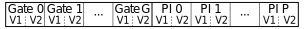
\includegraphics[width=\columnwidth]{figures/fig_gpu_state_structure.pdf}
\caption{The base data structure of GPU fault simulation is the circuit state, consisting of the $V_1$ and $V_2$ values of each gate output and primary input.
%
Each circuit state (either fault-free or faulty, for test vectors $V_1$ and $V_2$) is stored in a packed format, consisting first of the topologically-sorted gate output values, followed by the primary input values, with two bits per value.}
\label{fig:trax_gpu_state_structure}
\end{figure}
%\vskip 0.5em%

The third data structure is a lookup table for gate evaluation, a very frequent operation.
%
As previously mentioned, gates are restricted to one or two inputs, making it very simple to craft a lookup table to perform the gate evaluation.
%
The output value of a gate depends on the gate type and the two input values.
%
With eight primitive gate types (three bits) and two input values (two bits each), seven bits can be used to uniquely determine the output of a gate.
%
The gate-evaluation lookup table, therefore, contains $2^7 = 128$ values.
%
The one-input gates (the buffer and the inverter) only have four possible input combinations instead of 16, meaning that some of these values in the lookup table are redundant, but are maintained in the interest of lookup table regularity.
%
The gate-evaluation lookup table is stored in the GPU constants memory, which is a high-speed cached memory, and permits penalty-free parallel access by multiple threads.
%
The index into the lookup table is constructed from the gate type and the two input values, resulting in a seven-bit value, denoted as:

\begin{verbatim}
index = (gate.type << 4) | (in1_value << 2) | (in2_value)
\end{verbatim}

\subsubsection{Kernel 1 - Fault-Free Circuit Simulation}
\label{sec:trax_gpu_k1}

The first step of the fault simulation process is to compute the fault-free circuit states for all two-vector tests.
%
This is accomplished by Kernel 1 in the implementation, which assigns one GPU thread per test.
%
Before launching the GPU kernel, memory is first allocated to store one circuit state per test.
%
Each circuit state is then initialized with the proper test input values, with \textit{X} values assigned to all gate outputs.
%
The pseudocode of Kernel 1 is shown in Algorithm~\ref{alg:trax_gpu_k1}, and a graphical representation is shown in Figure~\ref{fig:trax_gpu_k1}.

\begin{algorithm}
\centering
\caption[GPU Kernel 1: Fault-Free Circuit Simulation]{-- Kernel 1: Fault-Free Circuit Simulation}
\label{alg:trax_gpu_k1}
\begin{algorithmic}[1]
\STATE testID = (blockID $\times$ BLOCKSIZE) + threadID
\IF{testID $<$ numTests}
  \STATE myState = allStates + (bytesPerState $\times$ testID)

  \COMMENT{iterate over all gates in topological order}
  \FOR{gateID = 0 \TO (numGates - 1)}
    \STATE cudaFaultSimCore(gates[gateID], myState)
  \ENDFOR
\ENDIF
\end{algorithmic}
\end{algorithm}

The Algorithm~\ref{alg:trax_gpu_k1} kernel is very simple, with each thread first computing its \verb+testID+ value (line 1 in Algorithm~\ref{alg:trax_gpu_k1}), and only continuing if it is less than the total number of two-input tests (line 2).
%
In line 3, the kernel generates a pointer into the state memory for its corresponding test.
%
Next, the kernel loops over all gates (lines 4-6), making one call to the \verb+cudaFaultSimCore()+ kernel function (line 5) per gate, which performs the actual simulation and assigns the gate output \verb+v1+ and \verb+v2+ values back into the thread circuit state.
%
Due to the topological sorting of gates, all threads evaluate the same gate at the same time, thereby staying in lock-step, and thus avoiding branch divergence.
%
After Kernel 1 finishes execution, the fault-free circuit states array has been filled with the fault-free circuit values for every test.

%\vskip 0.5em%
\begin{figure}[hbtp]
\centering
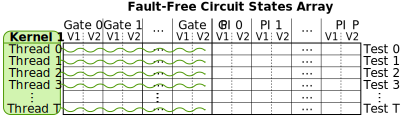
\includegraphics[width=\linewidth]{fig_gpu_k1}
\caption{Kernel 1 uses one GPU thread per two-vector test, with each thread performing a complete circuit simulation of all gates in the presence of the specific test.}
\label{fig:trax_gpu_k1}
\end{figure}
%\vskip 0.5em%

\subsubsection{Kernel function: {\tt cudaFaultSimCore()}}
\label{sec:trax_gpu_cuda_fault_sim_core}
This function is the core of the GPU fault simulator, and is called from both Kernel 1 (fault-free circuit simulation) and Kernel 3 (faulty circuit simulation).
%
The function is called once for each gate evaluation, and is described by the pseudocode in Algorithm~\ref{alg:trax_gpu_cudaFaultSimCore}.

\begin{algorithm}
\centering
\caption[GPU Kernel Function: \texttt{cudaFaultSimCore(gate, myState)}]{-- Kernel Function: \texttt{cudaFaultSimCore(gate, myState)}}
\label{alg:trax_gpu_cudaFaultSimCore}
\begin{algorithmic}[1]
\STATE in1v1 = myState[gate.in1 $\times$ 2]
\STATE in2v1 = myState[gate.in2 $\times$ 2]
\STATE in1v2 = myState[gate.in1 $\times$ 2 + 1]
\STATE in2v2 = myState[gate.in2 $\times$ 2 + 1]
\STATE v1 = gateEval(gate.type, in1v1, in2v1)
\STATE v2 = gateEval(gate.type, in1v2, in2v2)
\IF{hazardProduced(gate.type, in1v1, in1v2, in2v1, in2v2)}
  \STATE v2 = H
\ENDIF
\STATE myState[gate.id $\times$ 2] = v1
\STATE myState[gate.id $\times$ 2 + 1] = v2
\end{algorithmic}
\end{algorithm}

In \verb+cudaFaultSimCore()+, the input values to the current gate are loaded from the \verb+myState+ array in lines 1-4, and are used to compute the gate outputs to vector 1 and vector 2 (\verb+v1+ and \verb+v2+, respectively, in lines 5 and 6) using the gate evaluation lookup table.
%
The four input values are then used in line 7 to determine if a hazard is produced at the output of this gate, and if so, the value of \verb+v2+ is set equal to \textit{H} (line 8).
%
Finally, the \verb+myState+ array is updated with the computed gate-output values \verb+v1+ and \verb+v2+ in lines 10 and 11.

\subsubsection{Kernel 2 - Fault Activation Detection}
\label{sec:trax_gpu_k2}

In general, each two-vector test will activate only a subset of faults in the circuit, and the total fault simulation runtime can be reduced by simulating only the activated faults.
%
Although a TRAX fault, in theory, can also be activated by noise, we only consider here the following two situations:
\begin{enumerate}
\item A conventional gate output transition, either rising or falling.
%
An individual TRAX fault is either a ``slow to rise'' (STR) or a ``slow to fall'' (STF) fault, and in this activation situation, can only be activated by the corresponding gate output transition.
%
\item A hazard is present at the gate output, due to either hazard-causing inputs to the gate, or due to a hazard input value propagating through the gate.
%
There is no differentiating STR versus STF in this case since a hazard implies both a potential rising and falling transition.
\end{enumerate}

Each gate has two potential TRAX faults (a STR and STF fault), as shown in Figure~\ref{fig:trax_gpu_k2}.
%
The GPU fault simulator considers each fault independently, including the two faults belonging to a particular gate, using a separate thread for each fault.
%
Even in the situation where there is a hazard value at a gate output, which would activate both the STR as well as the STF fault, each GPU thread in Kernel 2 only considers a single fault.

Kernel 2 analyzes the fault-free circuit states array (generated by Kernel 1) to determine which faults are activated by which tests, and therefore need to be fault simulated to determine the output errors generated by the activated fault, if any.
%
Before launching the GPU kernel, the GPU memory is allocated to store a one-bit flag for each fault/test, indicating whether or not the fault is activated by the test (with a default value of ``not activated'').
%
Kernel 2 allocates one thread per fault, and each thread checks all tests to determine which tests activate its corresponding fault.

\begin{algorithm}
\centering
\caption[GPU Kernel 2: Fault Activation Detection]{-- Kernel 2: Fault Activation Detection}
\label{alg:trax_gpu_k2}
\begin{algorithmic}[1]
\STATE faultID = (blockID $\times$ BLOCKSIZE) + threadID
\IF{faultID $<$ numFaults}
  \STATE gateID = faultID / 2
  \COMMENT{two faults per gate}
  \STATE risingFault = faultID \% 2
  \COMMENT{even = STF, odd = STR}
  \FOR{testID = 0 \TO (numTests - 1)}
    \STATE myState = allStates + (bytesPerState $\times$ testID)
    \STATE v1 = myState[gateID $\times$ 2]
    \STATE v2 = myState[gateID $\times$ 2 + 1]
    \IF{(risingFault \AND (v1 =\,= 0) \AND (v2 =\,= 1)) \OR\\(\NOT risingFault \AND (v1 =\,= 1) \AND (v2 =\,= 0)) \OR\\(v2 =\,= H) )}
      \STATE markActivated(faultID, testID)
    \ENDIF
  \ENDFOR
\ENDIF
\end{algorithmic}
\end{algorithm}

Kernel 2 is described by the pseudocode in Algorithm~\ref{alg:trax_gpu_k2}.
%
Each thread of Kernel 2 first computes its \verb+faultID+ value (line 1) and only continues execution if it is less than the total number of faults (line 2).
%
The kernel computes the corresponding \verb+gateID+ (line 3) and determines in line 4 if its fault is an STR or STF fault (STF faults have an even \verb+faultID+ while STR faults have an odd \verb+faultID+).
%
Each GPU thread iterates over all tests (lines 5-12) and analyzes the \verb+v1+ and \verb+v2+ values at the fault site (lines 7-8).
%
The first two clauses of the if-conditional in line 9 check for the conventional activation involving a rising or falling transition affecting an STR or STF fault, respectively.
%
The final clause checks for the unique TRAX activation condition, where there is a hazard at the gate output.
%
If any of these conditions occur, the thread marks this fault as activated by this test in line 10.
%
A graphical representation of Kernel 2 is shown in Figure~\ref{fig:trax_gpu_k2}.

%\vskip 0.5em%
\begin{figure}[hbtp]
\centering
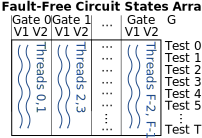
\includegraphics[width=0.5\columnwidth]{fig_gpu_k2}
\caption{Kernel 2 allocates two GPU threads per gate (one each for the STR and STF faults of the gate), where each thread analyzes the data for one gate in the fault-free circuit states array from Kernel 1 to determine which tests cause fault activation.}
\label{fig:trax_gpu_k2}
\end{figure}
%\vskip 0.5em%

After Kernel 2 has finished, the resulting fault activation information is transferred to the CPU for further processing, specifically to create three condensed arrays of fault activation data, as shown in Figure~\ref{fig:trax_gpu_activations_output}.
%
For each fault, in order, the activating \verb+testID+ values are all stored into the activating test IDs array.
%
Second, the total number of activations for each fault is recorded into the second array.
%
Finally, the fault activation counts are used to compute ``fault activation offsets'' for the faults, which determines the starting position of the \verb+testID+ values for the fault in the activating \verb+testIDs+ array.
%
These three arrays are used by the threads of Kernel 3 to identify which tests must be fault simulated.

%\vskip 0.5em%
\begin{figure}[hbtp]
\centering
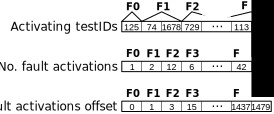
\includegraphics[width=0.8\columnwidth]{fig_gpu_activations_output}
\caption{The fault activation information generated by Kernel 2 is post-processed into the three arrays illustrated here, each of which is used by the threads of Kernel 3.}
\label{fig:trax_gpu_activations_output}
\end{figure}
%\vskip 0.5em%

\subsubsection{Kernel 3 - Fault-Effect Propagation}
\label{sec:trax_gpu_k3}

The final step of the fault simulation process is to determine how each activated fault affects the circuit primary outputs, with the end goal of finding which faults are detected by which tests.
%
Naturally, faults that are not activated by a given test will not be detected, so the fault simulator only performs fault simulation for activated faults for the tests that activate them, significantly reducing the required computation time.

In general, fault simulation is very similar to the fault-free circuit simulation of Kernel 1, which is the reason that the \verb+cudaFaultSimCore()+ function was created, enabling it to be used for both purposes.
%
However, there is one crucial difference here, in that the activated fault site must be identified as producing the output value \textit{X} (according to the TRAX fault model).
%
After this activation, fault simulation continues as in Kernel 1, as a gate-by-gate re-evaluation of the circuit.

Additionally, an optimization called ``skip ahead'' is used here to accelerate the parallel fault simulation.
%
Given that the circuit netlist gates are stored in topological order, an activated fault at gate $n$ cannot affect any gates that come before it, meaning that gate re-evaluation can simply start at gate $n+1$ and proceed to simulate the remaining gates in order.
%
While this optimization results in minimal time reduction for faults occurring early in the topological order, a significant amount of time reduction is observed for gates occurring later in the order.

Due to the fact that the concurrent simulation of different faults would require each thread to start at a different location in the gate ordering (unlike in Kernel 1, where all faults start at \verb+gateID=0+ and proceed in lock-step), Kernel 3 is designed to simulate the activations and fault-effect (i.e., \textit{X} value) propagations of a single fault for all activating two-vector tests, requiring one invocation of Kernel 3 for each fault in the circuit.
%
While this incurs a small amount of overhead for each kernel invocation, there are significant advantages to this approach, including enabling the skip-ahead optimization, avoiding branch-divergence between threads simulating different fault sites, and, especially, limiting the amount of memory required for Kernel 3.
%
The pseudocode of Kernel 3 is shown in Algorithm~\ref{alg:trax_gpu_k3}, and a graphical representation is given in Figure~\ref{fig:trax_gpu_k3}.

\begin{algorithm}
\centering
\caption[GPU Kernel 3: Fault-Effect Propagation]{-- Kernel 3: Fault-Effect Propagation}
\label{alg:trax_gpu_k3}
\begin{algorithmic}[1]
\STATE testOffset = (blockID $\times$ BLOCKSIZE) + threadID
\STATE faultOffset = faultActivationsOffset[faultID]
\IF{testOffset $<$ numFaultActivations[faultID]}
  \STATE testID = activatingTestIDs[faultOffset + testOffset]
  \STATE myState = allStates + (bytesPerState $\times$ testID)
  \STATE myGateID = faultID / 2
  \COMMENT{two faults per gate}
  \STATE myState[myGateID $\times$ 2 + 1] = X
  \COMMENT{activate the fault}

  \COMMENT{Simulation starts with the next gate}
  \FOR{gateID = (myGateID + 1) \TO (numGates - 1)}
    \STATE gate = gates[gateID]
    \STATE cudaFaultSimCore(gate, myState)
    \IF{gate.isOutput \AND myState[gateID $\times$ 2 + 1] =\,= X}
      \STATE markFaultDetected(faultID, testID)
    \ENDIF
  \ENDFOR
\ENDIF
\end{algorithmic}
\end{algorithm}

%\vskip 0.5em%
\begin{figure}[hbtp]
\centering
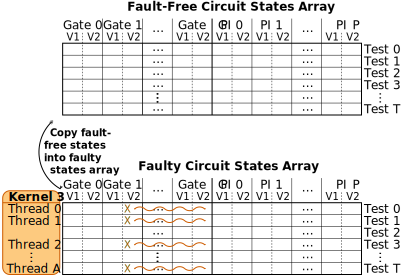
\includegraphics[width=\linewidth]{fig_gpu_k3}
\caption{Kernel 3 is invoked once per fault, and allocates one GPU thread per activated fault, which is designated by injecting an X value at the fault site and then simulating those gates that follow the fault site in the topologically-ordered list.}
\label{fig:trax_gpu_k3}
\end{figure}
%\vskip 0.5em%

Under this scheme, the GPU maintains in memory the fault-free circuit states from Kernel 1 (one state for each two-vector test).
%
For each invocation of Kernel 3 (for each fault to be simulated), the GPU makes a device-to-device memory copy of the fault-free circuit states to a temporary ``faulty circuit states'' memory location.
%
This is a constant amount of memory and does not depend on or scale with the number of activating tests for a given fault.

Each thread of Kernel 3 first computes its \verb+testOffset+ and \verb+faultOffset+ (lines 1-2) and only continues execution if the test offset is less than the total number of activations for this fault (line 3).
%
Kernel 3 uses the arrays shown in Figure~\ref{fig:trax_gpu_activations_output} to determine the corresponding \verb+testID+ (line 4), which serves as an index into the faulty circuit states array.
%
The gate corresponding to the current fault is determined (line 6), and the fault is activated by injecting an \textit{X} value at the fault site (line 7).
%
As part of the skip-ahead optimization, the gate loop in line 8 starts with \verb+gateID+ equal to the next gate after the fault site gate, simulating (line 10) each remaining gate in turn.
%
If a gate drives a circuit primary output and has an \textit{X} value as output (line 11), the fault has been detected, and the kernel records this in the fault dictionary data structure in line 12.

Given that the final output of the fault simulation (the pass/fail dictionary data) is a single bit for each fault/test pair, it would be inefficient to copy the complete faulty circuit states array from GPU to CPU after each invocation of Kernel 3, only to have the CPU determine the pass/fail bits from the circuit states, discarding a majority of the transferred data.
%
Instead, the fault dictionary data structure is created in GPU memory before any invocations of Kernel 3, initialized to have no faults marked as detected.
%
As each fault activation is simulated, the fault dictionary data structure in the GPU memory is updated with the fault detection status.
%
After all faults are simulated, the completed fault dictionary is finally transferred from GPU to CPU, where it is then copied to non-volatile memory.

In summary, fault dictionaries are indispensable for performing on-chip diagnosis but require significant computational resources to construct.
%
The inherent parallelism of fault simulation makes it an ideal candidate for acceleration through the use of a GPU.
%
The CUDA-based GPU-accelerated fault simulator for TRAX faults described here is a straightforward and efficient way to perform the necessary fault simulations required to generate a TRAX fault dictionary, and will be shown to be practical in comparison with a commercial fault simulator by experiments in Section~\ref{sec:trax_exp_gpu}.


\section{Experiments}
\label{trax_exp}

Several experiments are performed to evaluate the TRAX fault model and GPU-accelerated fault simulation.
%
A gate-level simulation experiment comparing TF and TRAX fault responses is described in Section~\ref{sec:trax_exp_fault_effects}, and a series of experiments on various benchmark circuits are presented in Section \ref{sec:trax_exp_gpu}.

\subsection{Comparison of TRAX and TF Fault Effects}
\label{sec:trax_exp_fault_effects}

To further explore and validate the TRAX subsumption of TF fault responses, we perform a series of circuit simulation experiments on a number of benchmark and other circuits.
%
Fault simulation is used to determine the number of tests that detect each simulated fault, as well as determine the count of failing circuit outputs.
%
This fault simulation is performed for both TRAX and TF faults, for four different benchmark circuits.
%
The resulting counts of fault detecting tests and failing output bits are normalized for each circuit to permit cross-circuit comparison.

%\vskip 0.2em%
\begin{figure}[hbtp]
\centering
\includegraphics[width=0.9\columnwidth]{fig_norm_output_count}
\caption{Each point above represents a single fault, positioned to indicate the relative count of failing circuit outputs between TRAX and TF fault simulation, for four different benchmark circuits.
%
The results demonstrate that TRAX fault effects subsume TF fault effects.}
\label{fig:norm_output_count}
\end{figure}
%\vskip 0.5em%

%\vskip 0.2em%
\begin{figure}[hbtp]
\centering
\includegraphics[width=0.9\columnwidth]{fig_norm_detection_count}
\caption[Each point above represents a single fault, positioned to indicate the relative count of failing tests between TRAX and TF fault simulation, for four different benchmark circuits.
%
The results demonstrate that TRAX fault detections subsume TF fault detections.]{Each point above represents a single fault, positioned to indicate the relative count of failing tests between TRAX and TF fault simulation, for four different benchmark circuits.
%
The results demonstrate that TRAX fault detections subsume TF fault detections.
%
(Note that it is possible that the corresponding TF and TRAX faults are failing at different outputs even though TRAX has the same or larger count.)}
\label{fig:norm_detection_count}
\end{figure}
%\vskip 0.5em%

Figures~\ref{fig:norm_output_count} and \ref{fig:norm_detection_count} show a scatter plot comparison between TRAX and TF fault responses for each simulated fault.
%
Each point in these two figures is a single simulated fault, where the position is determined by the normalized count of failing outputs (Figure~\ref{fig:norm_output_count}) or detecting tests (Figure~\ref{fig:norm_detection_count}) for TRAX and TF simulations of that fault.
%
A line is drawn to indicate where TRAX and TF have equal counts.
%
We observe that for both detections and failing output count, for every fault, the TRAX behavior subsumes the TF behavior, as made evident by no faults falling below the indicated line.

\subsection{TRAX Fault Simulation Acceleration}
\label{sec:trax_exp_gpu}

A series of experiments evaluate both the accuracy and acceleration of the GPU TRAX fault simulator.
%
Due to the unavailability of a TRAX-compatible commercial fault simulator, a single-threaded CPU reference implementation is used to verify the accuracy of the GPU fault simulator using two-vector tests created by a commercial ATPG tool targeting conventional transition faults.
%
For all circuits and two-vector tests, there are no discrepancies between the reference implementation and the accelerated GPU implementation.

To evaluate runtime performance, the GPU simulator is compared to a commercial fault simulation tool that is used with conventional transition faults.
%
Although the commercial tool is unable to fully implement the features of the TRAX fault model (and instead simulates transition faults), a comparison of the two execution times is worthwhile.
%
As previously mentioned, each large gate has been replaced by an equivalent subcircuit of two-input gates to simplify the GPU fault simulation.
%
The set of faults to simulate is generated from the original netlist (before large gates are replaced), and this fault set is provided to both the commercial tool and the GPU fault simulator to ensure a fair comparison.
%
Because the two-vector test set is generated as part of the commercial tool ATPG process, the tool writes the test set to disk so it can be imported into the GPU fault simulator, ensuring that the same tests are used for both fault simulation tools.
%
The commercial fault simulation tool is running on a 2.2 GHz Xeon E5-4620 (single-threaded fault simulation), and the GPU fault simulation is running on a Nvidia GTX-1080 GPU.

%\vskip 0.5em%
\begin{table}[hbtp]
\centering
\begin{tabular*}{1.0\columnwidth}{@{\extracolsep{\fill}}|l|rr|r|rr|}
\hline
                                &\multicolumn{2}{c|}{GPU (s)}       &\multicolumn{1}{c|}{CPU (s)}   &\multicolumn{2}{c|}{Speedup}\\
\hline
Circuit (No. gates, No. tests)  &TRAX       &TF                     &TF                             &TRAX   &TF\\
\hline
c432 (208, 37)                  &0.148      &0.123                  &1.895                          &12.76  &15.37\\
c499 (246, 71)                  &0.130      &0.124                  &2.469                          &19.00  &19.88\\
c1355 (558, 106)                &0.281      &0.243                  &4.809                          &17.11  &19.79\\
c1908 (368, 64)                 &0.154      &0.144                  &2.376                          &15.45  &16.48\\
c2670 (1,168, 67)               &0.658      &0.539                  &8.779                          &13.35  &16.30\\
c3540 (1,512, 128)              &1.181      &0.942                  &12.346                         &10.46  &13.11\\
c5315 (2,740, 85)               &3.177      &2.444                  &23.691                         &7.46   &9.69\\
c7552 (3,223, 84)               &4.750      &3.582                  &29.963                         &6.31   &8.36\\
\hline
b12 (1,336, 80)                 &0.641      &0.506                  &7.375                          &11.50  &14.58\\
b14\_opt (6,878, 345)           &39.377     &23.439                 &201.311                        &5.11   &8.59\\
b14 (10,682, 657)               &201.269    &77.986                 &1,009.105                      &5.01   &12.94\\
b15 (9,877, 407)                &81.045     &46.432                 &503.040                        &6.21   &10.83\\
b17\_opt (30,396, 600)          &907.294    &453.962                &4,996.472                      &5.51   &11.01\\
b18\_opt (90,729, 704)          &9,015.342  &4,551.655              &51,812.517                     &5.75   &11.38\\
b22 (32,247, 554)               &1,676.197  &558.607                &5,303.097                      &3.16   &9.49\\
\hline
L2B (12,222, 90)                &83.655     &58.413                 &550.146                        &6.58   &9.42\\
NCU (78,677, 211)               &1,755.930  &1,243.913              &15,033.808                     &8.56   &12.09\\
\hline
epflDiv (101,603, 612)          &17,198.853 &8,390.128              &50,236.483                     &2.92   &5.99\\
epflMult (50,504, 77)           &1,338.662  &1,026.140              &2,668.724                      &1.99   &2.60\\
epflSqrt (41,042, 161)          &1,185.846  &810.855                &2,945.845                      &2.48   &3.63\\
epflSquare (35,492, 79)         &661.580    &527.172                &1,404.470                      &2.12   &2.66\\
epflMemCtrl (82,538, 1,276)     &13,870.393 &8,427.150              &93,803.048                     &6.76   &11.13\\
\hline
\multicolumn{4}{|r|}{Average:}                                                                      &7.98   &11.15\\
\multicolumn{4}{|r|}{Maximum:}                                                                      &19.00  &19.88\\
\hline
\end{tabular*}
\caption{Fault simulation (with no fault dropping) is performed using the GPU fault simulator (for TRAX and TF models) as well as a commercial fault simulator (TF model only) in order to compare the runtime of each.
%
The speedup results compare the GPU TRAX and TF runtimes with the CPU (commercial tool) TF runtimes.}
\label{table:trax_exp_gpu_runtime_comparison}
\end{table}
%\vskip 0.5em%

Comparative fault simulation results (without fault dropping) are shown in Table~\ref{table:trax_exp_gpu_runtime_comparison}.
%
The GPU fault simulator can perform both TF and TRAX fault simulation, while the commercial tool can only perform TF fault simulation.
%
The GPU and commercial-tool runtimes are reported in seconds, and the speedup comparisons are shown in the final two columns.
%
The highest speedup is achieved for the smaller ISCAS85~\cite{brglez85} benchmark circuits, with a declining speedup as circuit size increases.
%
The EPFL circuits~\cite{epfl}, in addition to being some of the largest circuits analyzed, generally show the least speedup.
%
Overall, when comparing the TF runtimes between the GPU and CPU implementations, the average speedup is 11.15x with a maximum speedup of 19.88x.
%
Due to the increased number of fault activations when performing TRAX fault simulation as compared to TF fault simulation, the TRAX fault simulations achieved less of a speedup than for TF.
%
For TRAX the average speedup achieved is 7.98x, with a maximum speedup of 19x.
%
When comparing GPU fault simulation runtimes for the TF and TRAX fault models, we observed that GPU TF fault simulation was 1.5x faster than TRAX fault simulation, on average.
%



\section{Summary}
\label{sec:trax_summary}

Targeting the gradual slowdowns of early-life and wear-out failures, the TRAX fault model is a new enhancement to the unspecified-transition fault model~\cite{pomeranz08}.
%
TRAX faults conservatively and efficiently capture all possible activation and propagation paths for a speed-degraded standard cell.
%
Whether activated by a conventional gate output transition or activated by a hazard, a TRAX fault generates an \textit{X} value that encompasses all possible transport delays through that gate.
%
Designed to subsume all potential delay fault effects, fault simulation has shown that the TRAX model does indeed subsume the fault effects of the TF model.
%
To counter the large amount of computation required to generate the fault dictionary, a GPU-accelerated fault simulation engine has been developed.
%
Fault simulation experiments show an average speed-up of nearly 8x for the GPU fault simulator when compared to a leading commercial tool.

